\section{Results}
\label{sec:results}

\begin{figure}
  % Requires \usepackage{graphicx}
  \begin{center}
	\begin{tabular}{ccc}
	  \parbox{30mm}{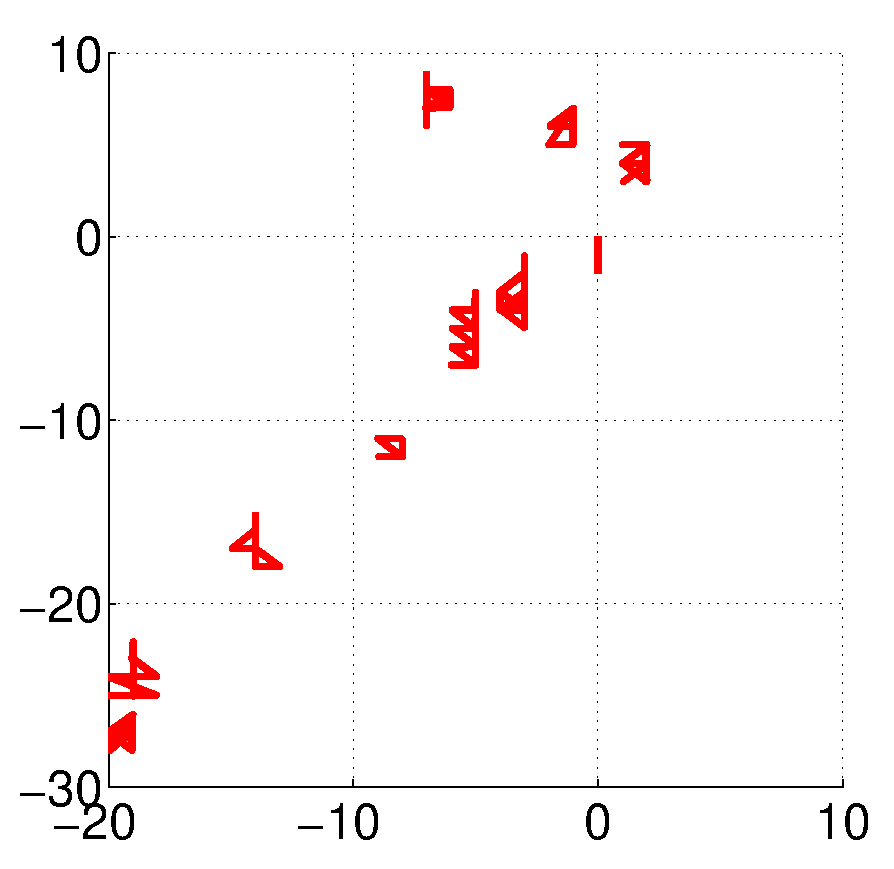
\includegraphics[width=30mm]{Figure/LeftEyeOpenLoop.eps}}  & \hspace{0.1cm} &
	  \parbox{30mm}{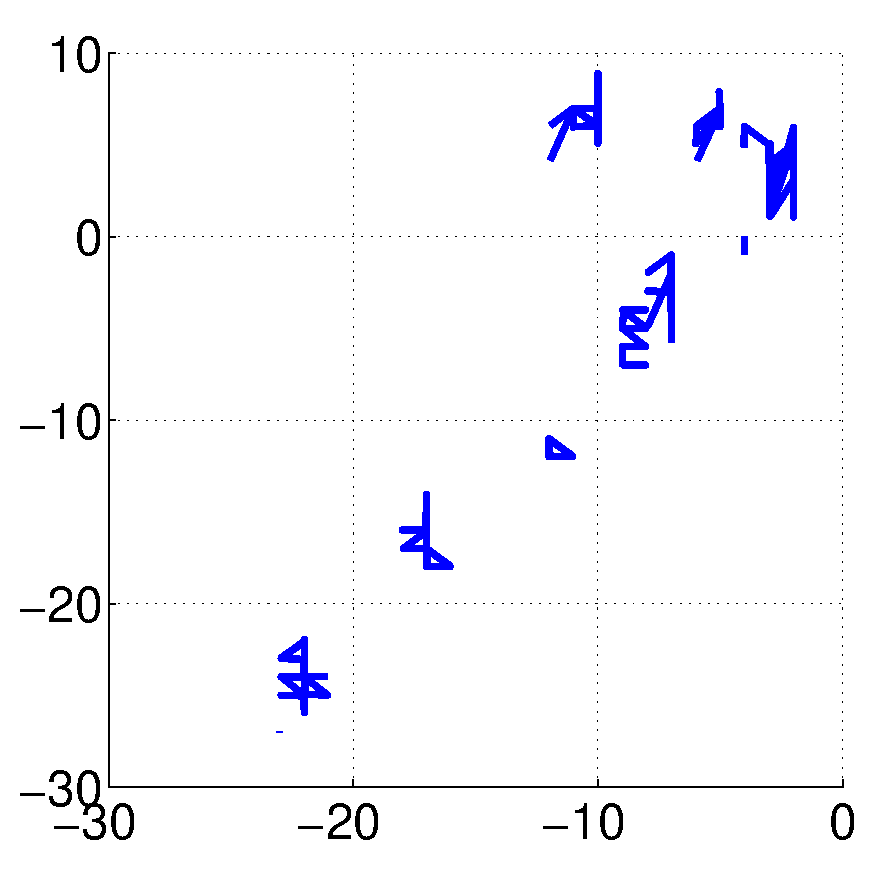
\includegraphics[width=30mm]{Figure/RightEyeOpenLoop.eps}}
	  \\
	  \parbox{30mm}{\centering Left eye } & \hspace{0.1cm} & \parbox{30mm}{\centering Right eye }
	  %	  \end{t\\
	  %	Top view & & Lateral view
  \end{tabular}
\end{center}
\caption{Open loop performance, for different choices of the redundant 
variable $q_{20}$ (image plane errors $\uhand$, in pixels). On the horizontal 
axis $u_r$ and $u_l$; vertical axis $v_r$ and $v_l$ (always in pixels).
The hand position in the image plane is represented 
by the small circles.  Each circle corresponds to a different open loop 
movement, i.e. a different value of $q_{20}$.
}\label{Fig:ImagePlaneOpenLoopErrors}
 \end{figure}

\begin{figure}
  % Requires \usepackage{graphicx}
  \begin{center}
	\begin{tabular}{ccc}
	  \parbox{30mm}{\includegraphics[width=30mm]{Figure/LeftEyeClosedLoop.eps}}  & \hspace{.1cm} &
	  \parbox{30mm}{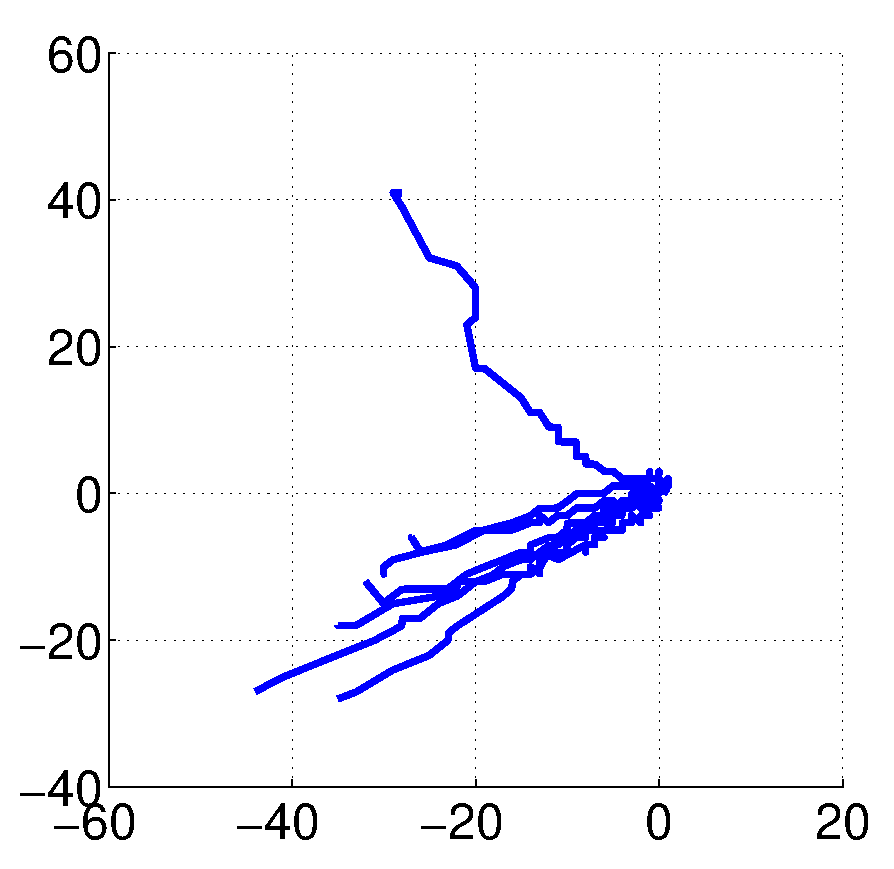
\includegraphics[width=30mm]{Figure/RightEyeClosedLoop.eps}}
	  \\
	  \parbox{30mm}{\centering Left eye } & \hspace{0.1cm} & \parbox{30mm}{\centering Right eye }
	  %	  \end{t\\
	  %	Top view & & Lateral view
  \end{tabular}
\end{center}
\caption{Traces of different closed loop control actions. Each trace correspond to a different Cartesian position of the target to be reached (which 
is always at the center of the image planes). All the traces end up in the image center thus indicating that the visual errors are completely eliminated by the closed loop controller.}\label{Fig:ImagePlaneClosedLoopErrors}
  \end{figure}


\begin{figure}
  % Requires \usepackage{graphicx}
  \begin{center}
	\begin{tabular}{ccc}
	  \parbox{30mm}{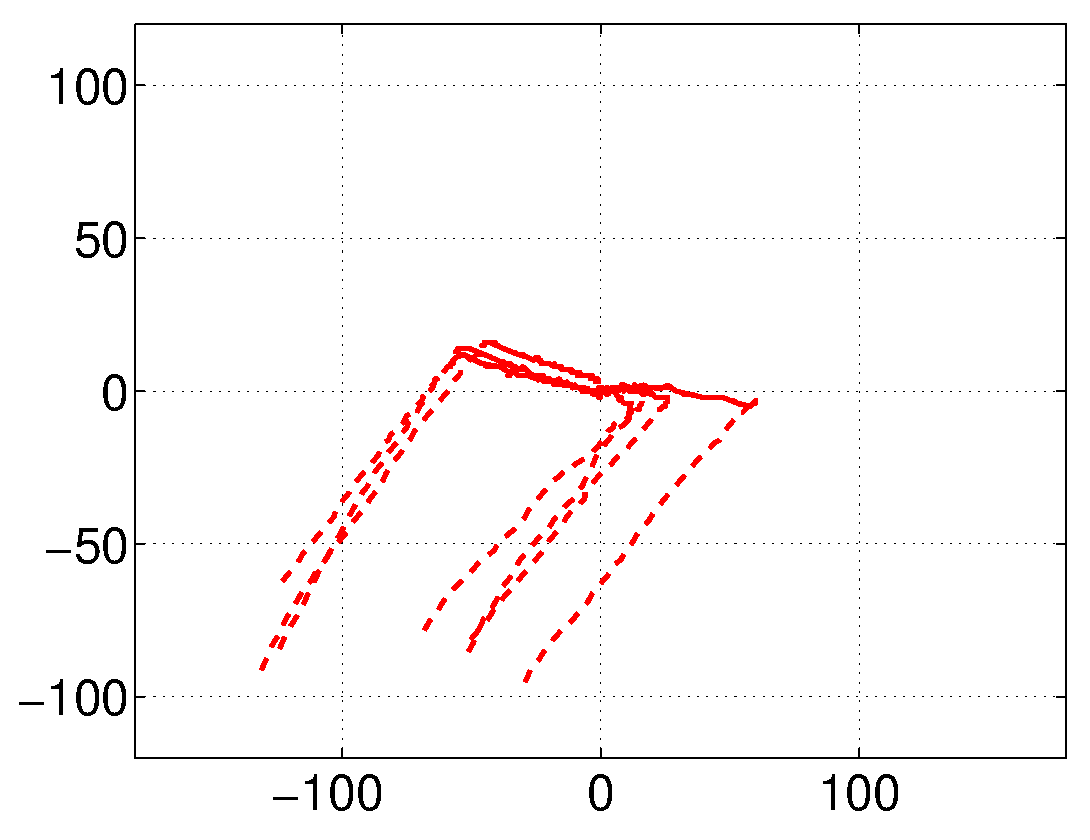
\includegraphics[width=30mm]{Figure/LeftEyeOpenClosedLoop.eps}}  & \hspace{.1cm} &
	  \parbox{30mm}{\includegraphics[width=30mm]{Figure/RightEyeOpenClosedLoop.eps}}
	  \\
	  \parbox{30mm}{\centering Left eye } & \hspace{.1cm} & \parbox{30mm}{\centering Right eye }
	  %	  \end{t\\
	  %	Top view & & Lateral view
  \end{tabular}
\end{center}
\caption{Movement of the hand on the image planes (320$\times$240)
during the execution of different reaching actions. 
Solid line: closed loop. Dashed trace: open loop. Clearly the open loop movement drives the hand to the target (the image centers) with a 
relatively small error. The closed loop phase reduces this error to zero.}\label{Fig:TimeResponseOpenClosedLoopErrors}
  \end{figure}
  
  \begin{figure}
  % Requires \usepackage{graphicx}
  \begin{center}
	\begin{tabular}{ccc}
	  \parbox{30mm}{\includegraphics[width=30mm]{Figure/LeftEyeOpenClosedLoopTimeResponse.eps}}  & \hspace{.1cm} &
	  \parbox{30mm}{\includegraphics[width=30mm]{Figure/RightEyeOpenClosedLoopTimeResponse.eps}}
	  \\
	  \parbox{30mm}{\centering Left eye } & \hspace{.1cm} & \parbox{50mm}{\centering Right eye }
	  %	  \end{t\\
	  %	Top view & & Lateral view
  \end{tabular}
\end{center}
\caption{Time response of the closed loop and open loop strategy. Solid lines: $u_r$ and $u_l$. Dashed lines: $v_r$ and $v_l$. Remarkably, the open loop phase is faster but does not drive the hand exactly on the target. The closed loop is slower but more accurate.}\label{Fig:TimeResponseOpenClosedLoop}
\end{figure}


In this section we report the results of the experiments we carried out
to quantify the performance of the reaching movements. Following the proposed 
strategy, in order to reach for the 
target we first need to fixate it, i.e. $\utarget = 0$. Using the available 
sensor (i.e. vision) the best we can do to precisely reach the target is 
moving the hand to the fixation point, i.e. 
${\uhand} \longrightarrow 0$. Clearly, the image plane distance 
$e=\| \uhand - \utarget \|$ can be used as a rough estimate of the reaching 
precision, i.e. of the Cartesian distance between the target to be reached 
and the position of the hand. %Specifically, assuming infinite resolution of 
%the camera sensor, if $e=0$ then the hand has exactly 
%reached the target.
%
%\subsection{Open Loop}

The first attempt to reach the target consists in using (\ref{Eq:reaching2})
to choose the arm configuration $\q_{arm}$ which brings the hand to the center 
of the image planes. Clearly, if the forward 
kinematic function (\ref{Eq:forward}) were perfectly represented and if the 
target were reachable, then we would have 
$\mathbf x_{hand} =  \mathbf x_{target}$, which implies that the target-hand 
Cartesian distance is zero, $e=0$ (see Section \ref{sec:reaching} 
for details). In practice, the model (\ref{Eq:forward}) cannot exactly 
represent the system's kinematics
%\footnote{Part of the representational 
%errors are related to the neural model approximating the kinematic function. 
%Part are due to the mechanical backlash of the structure.}
, therefore it is 
not guaranteed that after the movement 
execution $e=0$. Figure \ref{Fig:ImagePlaneOpenLoopErrors}
shows the image plane errors after the execution of the open loop movement. 
The plot has been obtained by fixating a target and performing a series of 
open loop movements. Each open loop 
movement was different because (\ref{Eq:reaching2}) was solved 
by choosing a different value $q_{20}$.

%\subsection{Closed Loop}
%
The residual image plane errors can be reduced 
by a visual closed loop control strategy. This control strategy moves the 
arm to progressively 
drive the hand position in the image planes ($\uhand$) to zero. Figures
\ref{Fig:ImagePlaneClosedLoopErrors}, %\ref{Fig:TimeResponseClosedLoopErrors}, 
\ref{Fig:TimeResponseOpenClosedLoopErrors} and \ref{Fig:TimeResponseOpenClosedLoop}  
show how the hand is actually driven to the 
exact image center in both the image planes. The closed loop controller 
improves the accuracy of the reaching movement, but at the cost of a slower 
execution speed (see Figure \ref{Fig:TimeResponseOpenClosedLoop}). 
Moreover, it is important to notice 
the quasi-linearity of the path followed by the hand 
(see Figure \ref{Fig:ImagePlaneClosedLoopErrors}). This linearity denotes 
a good accuracy of the learned Jacobian.

%%%% this figure has been removed to save space
%% \begin{figure}
%%   % Requires \usepackage{graphicx}
%%   \begin{center}
%% 	\begin{tabular}{ccc}
%% 	  \parbox{30mm}{\includegraphics[width=30mm]{Figure/TimeReponseLeftClosedLoop.eps}}  & \hspace{.1cm} &
%% 	  \parbox{30mm}{\includegraphics[width=30mm]{Figure/TimeReponseRightClosedLoop.eps}}
%% 	  \\
%% 	  \parbox{30mm}{\centering Left eye } & \hspace{0.1cm} & \parbox{30mm}{\centering Right eye }
%% 	  %	  \end{t\\
%% 	  %	Top view & & Lateral view
%%   \end{tabular}
%% \end{center}
%% \caption{Time response of the closed loop controller. Solid lines: hand horizontal position in the left ($u_l$) and right ($u_r$). Dashed lines: vertical position, $v_l$ and $v_r$.}\label{Fig:TimeResponseClosedLoopErrors}
%%   \end{figure}